\documentclass[tikz,border=8pt]{standalone}
\usepackage{amsmath}
\usepackage{amssymb}
\usetikzlibrary{arrows.meta,calc,decorations.pathreplacing,decorations.markings,decorations.pathmorphing,patterns,shapes.geometric,positioning}

\begin{document}
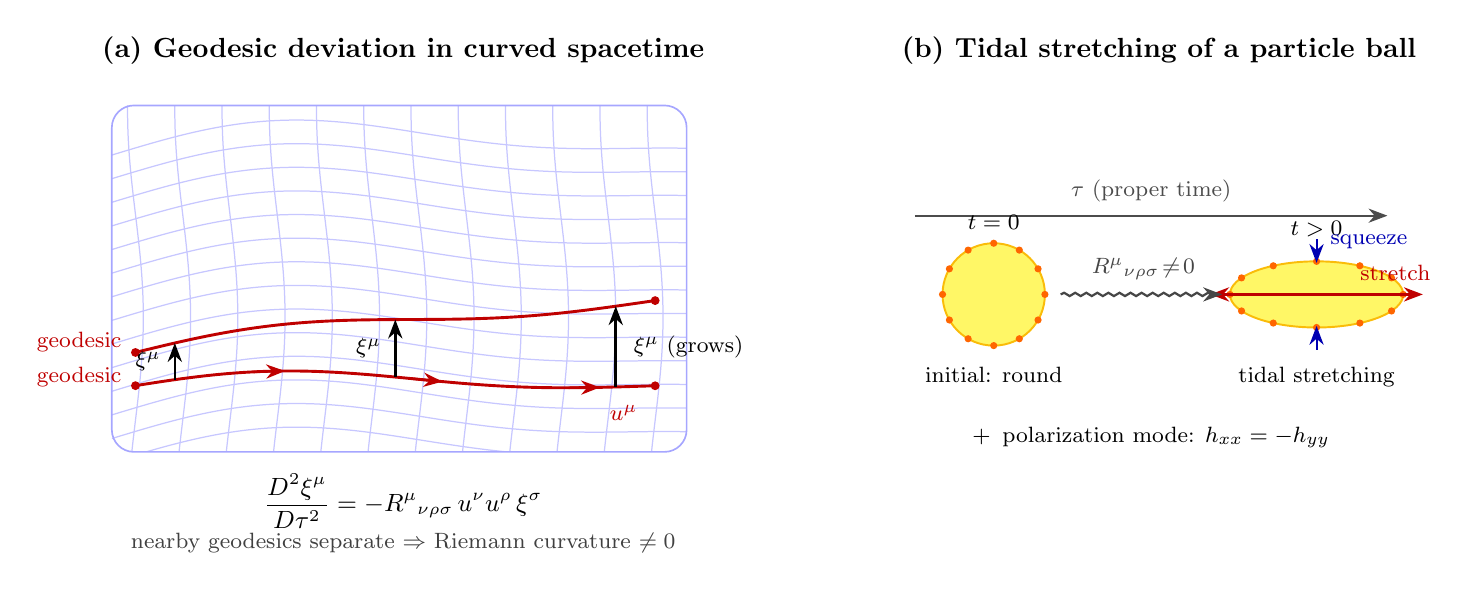
\begin{tikzpicture}[>={Stealth[length=2.4mm,width=1.8mm]},line width=0.7pt,font=\small]

% ==============================================================
% LEFT PANEL : Curved 2D-surface with two nearby geodesics
% and the deviation vector xi
% ==============================================================
\begin{scope}[xshift=0cm,yshift=0cm]

  \node[font=\bfseries,anchor=north] at (3.4,5.0) {(a) Geodesic deviation in curved spacetime};

  % --- Light-blue curved sheet drawn as a stack of curves
  \begin{scope}
    \clip (-0.3,-0.4) rectangle (7.0,4.0);
    % horizontal-ish curves (gridlines)
    \foreach \yv in {-0.2,0.1,0.4,0.7,1.0,1.3,1.6,1.9,2.2,2.5,2.8,3.1,3.4,3.7}{
      \draw[blue!22!white,line width=0.45pt,smooth,samples=60,domain=-0.3:7.0]
        plot (\x,{\yv + 0.16*sin(deg(\x*0.95)) - 0.022*(\x-3.3)*(\x-3.3)});
    }
    % vertical-ish curves
    \foreach \xv in {0.0,0.6,1.2,1.8,2.4,3.0,3.6,4.2,4.8,5.4,6.0,6.6}{
      \draw[blue!22!white,line width=0.45pt,smooth,samples=40,domain=-0.4:4.0]
        plot ({\xv + 0.10*sin(deg(\x*1.20))},\x);
    }
  \end{scope}

  % outline of the sheet
  \draw[blue!35!white,line width=0.6pt,rounded corners=8pt]
    (-0.3,-0.4) rectangle (7.0,4.0);

  % --- Two nearby geodesics, dark-red, that diverge as they go right
  % geodesic 1 (lower)
  \draw[red!75!black,line width=1.05pt,smooth,samples=80,domain=0.0:6.6]
    plot (\x,{0.55 + 0.10*sin(deg(\x*0.95)) - 0.010*(\x-3.3)*(\x-3.3)});
  % geodesic 2 (upper)
  \draw[red!75!black,line width=1.05pt,smooth,samples=80,domain=0.0:6.6]
    plot (\x,{0.95 + 0.10*\x + 0.10*sin(deg(\x*0.95)) - 0.008*(\x-3.3)*(\x-3.3)});

  % Endpoint dots (start)
  \fill[red!75!black] (0.0,{0.55 + 0.10*sin(0) - 0.010*(0-3.3)*(0-3.3)}) circle (1.6pt);
  \fill[red!75!black] (0.0,{0.95 + 0.10*0.0 + 0.10*sin(0) - 0.008*(0-3.3)*(0-3.3)}) circle (1.6pt);
  % End dots
  \fill[red!75!black] (6.6,{0.55 + 0.10*sin(deg(6.6*0.95)) - 0.010*(6.6-3.3)*(6.6-3.3)}) circle (1.6pt);
  \fill[red!75!black] (6.6,{0.95 + 0.10*6.6 + 0.10*sin(deg(6.6*0.95)) - 0.008*(6.6-3.3)*(6.6-3.3)}) circle (1.6pt);

  % small arrows along lower geodesic (4-velocity u^mu)
  \foreach \xv in {1.5,3.5,5.5}{
     \pgfmathsetmacro{\yA}{0.55 + 0.10*sin(deg(\xv*0.95)) - 0.010*(\xv-3.3)*(\xv-3.3)}
     \pgfmathsetmacro{\xvB}{\xv+0.4}
     \pgfmathsetmacro{\yAA}{0.55 + 0.10*sin(deg((\xv+0.4)*0.95)) - 0.010*((\xv+0.4)-3.3)*((\xv+0.4)-3.3)}
     \draw[->,red!75!black,line width=0.9pt] (\xv,\yA) -- (\xvB,\yAA);
  }
  \node[red!75!black,font=\footnotesize] at (6.2,0.10) {$u^\mu$};

  % geodesic labels
  \node[red!75!black,anchor=east,font=\footnotesize] at (-0.05,0.55) {geodesic};
  \node[red!75!black,anchor=east,font=\footnotesize] at (-0.05,1.00) {geodesic};

  % ----- Deviation vectors xi^mu : at three time-slices -----
  % t=0 : small separation
  \pgfmathsetmacro{\xa}{0.5}
  \pgfmathsetmacro{\yaA}{0.55 + 0.10*sin(deg(\xa*0.95)) - 0.010*(\xa-3.3)*(\xa-3.3)}
  \pgfmathsetmacro{\yaB}{0.95 + 0.10*\xa + 0.10*sin(deg(\xa*0.95)) - 0.008*(\xa-3.3)*(\xa-3.3)}
  \draw[->,black,line width=0.9pt] (\xa,\yaA) -- (\xa,\yaB);

  % t=mid
  \pgfmathsetmacro{\xb}{3.3}
  \pgfmathsetmacro{\ybA}{0.55 + 0.10*sin(deg(\xb*0.95)) - 0.010*(\xb-3.3)*(\xb-3.3)}
  \pgfmathsetmacro{\ybB}{0.95 + 0.10*\xb + 0.10*sin(deg(\xb*0.95)) - 0.008*(\xb-3.3)*(\xb-3.3)}
  \draw[->,black,line width=0.9pt] (\xb,\ybA) -- (\xb,\ybB);

  % t=late
  \pgfmathsetmacro{\xc}{6.1}
  \pgfmathsetmacro{\ycA}{0.55 + 0.10*sin(deg(\xc*0.95)) - 0.010*(\xc-3.3)*(\xc-3.3)}
  \pgfmathsetmacro{\ycB}{0.95 + 0.10*\xc + 0.10*sin(deg(\xc*0.95)) - 0.008*(\xc-3.3)*(\xc-3.3)}
  \draw[->,black,line width=1.0pt] (\xc,\ycA) -- (\xc,\ycB);

  % xi labels
  \node[black,anchor=east,font=\footnotesize] at (\xa-0.05,{(\yaA+\yaB)/2}) {$\xi^\mu$};
  \node[black,anchor=east,font=\footnotesize] at (\xb-0.05,{(\ybA+\ybB)/2}) {$\xi^\mu$};
  \node[black,anchor=west,font=\footnotesize] at (\xc+0.10,{(\ycA+\ycB)/2}) {$\xi^\mu$ (grows)};

  % ----- Master formula -----
  \node[anchor=north,font=\small] at (3.4,-0.55)
    {$\dfrac{D^2 \xi^\mu}{D\tau^2}=-R^\mu{}_{\nu\rho\sigma}\,u^\nu u^\rho\,\xi^\sigma$};

  \node[anchor=north,font=\footnotesize,gray!50!black] at (3.4,-1.30)
    {nearby geodesics separate $\Rightarrow$ Riemann curvature $\neq 0$};

\end{scope}


% ==============================================================
% RIGHT PANEL : ball of test particles -> stretched ellipse
% ==============================================================
\begin{scope}[xshift=10.5cm,yshift=1.0cm]

  \node[font=\bfseries,anchor=north] at (2.5,4.0) {(b) Tidal stretching of a particle ball};

  % time arrow
  \draw[->,gray!60!black,line width=0.6pt] (-0.6,1.6) -- (5.4,1.6);
  \node[gray!60!black,font=\footnotesize,anchor=south] at (2.4,1.65) {$\tau$ (proper time)};

  % --- Initial: circle of test particles
  \fill[yellow!60,draw=yellow!50!orange,line width=0.7pt] (0.4,0.6) circle (0.65);
  \foreach \ang in {0,30,60,90,120,150,180,210,240,270,300,330}{
    \fill[orange!80!red] ($(0.4,0.6)+(\ang:0.65)$) circle (1.3pt);
  }
  \node[anchor=north,font=\footnotesize] at (0.4,-0.20) {initial: round};
  \node[anchor=south,font=\footnotesize] at (0.4,1.30) {$t=0$};

  % --- Final: stretched ellipse (yellow)
  \fill[yellow!60,draw=yellow!50!orange,line width=0.7pt]
    (4.5,0.6) ellipse (1.10 and 0.42);
  \foreach \ang in {0,30,60,90,120,150,180,210,240,270,300,330}{
    \fill[orange!80!red] ($(4.5,0.6)+({1.10*cos(\ang)},{0.42*sin(\ang)})$) circle (1.3pt);
  }
  \node[anchor=north,font=\footnotesize] at (4.5,-0.20) {tidal stretching};
  \node[anchor=south,font=\footnotesize] at (4.5,1.20) {$t>0$};

  % stretching arrows (red)
  \draw[->,red!75!black,line width=0.9pt] (4.5,0.6) -- (5.85,0.6);
  \draw[->,red!75!black,line width=0.9pt] (4.5,0.6) -- (3.15,0.6);
  % compression arrows (blue)
  \draw[->,blue!70!black,line width=0.7pt] (4.5,1.30) -- (4.5,1.0);
  \draw[->,blue!70!black,line width=0.7pt] (4.5,-0.10) -- (4.5,0.20);

  % labels
  \node[red!75!black,font=\footnotesize,anchor=south] at (5.5,0.65) {stretch};
  \node[blue!70!black,font=\footnotesize,anchor=south west] at (4.55,1.05) {squeeze};

  % connecting wavy arrow between two figures
  \draw[->,gray!55!black,line width=0.8pt,decorate,decoration={snake,segment length=4pt,amplitude=0.6pt,post length=2pt}]
    (1.25,0.6) -- (3.30,0.6);

  \node[gray!55!black,font=\footnotesize,anchor=south] at (2.30,0.66) {$R^\mu{}_{\nu\rho\sigma}\!\neq\!0$};

  % bottom note
  \node[anchor=north,font=\footnotesize] at (2.4,-0.95)
    {$+\,$ polarization mode: $h_{xx}=-h_{yy}$};

\end{scope}

\end{tikzpicture}
\end{document}
